\begin{figure}[t]
  \centering
  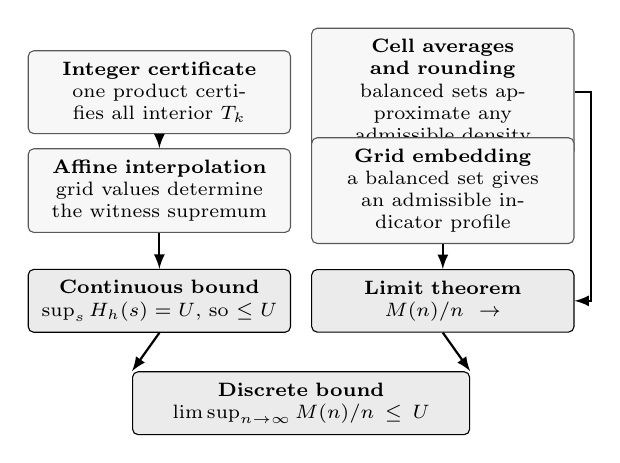
\begin{tikzpicture}[
    font=\scriptsize,
    >=latex,
    box/.style={draw=black!65, rounded corners=2pt, align=center,
      fill=black!3, text width=3.05cm, inner sep=4pt},
    claim/.style={box, draw=black, fill=black!8},
    path/.style={->, thick}
  ]
    \node[box] (digits) at (-1.80,0)
      {\textbf{Integer certificate}\\one product certifies all interior $T_k$};
    \node[box] (cells) at (1.80,0)
      {\textbf{Cell averages and rounding}\\balanced sets approximate any admissible density};
    \node[box] (affine) at (-1.80,-1.25)
      {\textbf{Affine interpolation}\\grid values determine the witness supremum};
    \node[box] (embed) at (1.80,-1.25)
      {\textbf{Grid embedding}\\a balanced set gives an admissible indicator profile};
    \node[claim] (cont) at (-1.80,-2.65)
      {\textbf{Continuous bound}\\$\sup_s H_h(s)=U$, so $\ct\le U$};
    \node[claim] (limit) at (1.80,-2.65)
      {\textbf{Limit theorem}\\$M(n)/n\to\ct$};
    \node[claim,text width=4.0cm] (disc) at (0,-3.95)
      {\textbf{Discrete bound}\\$\limsup_{n\to\infty} M(n)/n\le U$};
    \draw[path] (digits.south) -- (affine.north);
    \draw[path] (affine.south) -- (cont.north);
    \draw[path] (embed.south) -- (limit.north);
    \draw[path] (cells.east) -- ++(.21,0) |- (limit.east);
    \draw[path] (cont.south) -- (disc.north west);
    \draw[path] (limit.south) -- (disc.north east);
  \end{tikzpicture}
  \caption{The witness certifies an upper bound on the continuous infimum
  $\ct$. Rounding and grid embedding identify $\ct$ with the limit of the
  discrete minima. Both branches are formalized in Lean.}
  \label{fig:bridge}
  \Description{Two proof branches meet at the discrete bound. Packed
  coefficients and affine interpolation bound the witness supremum.
  Averaging and rounding give the upper half of the limit theorem, and
  embedding balanced sets as step functions gives the lower half.}
\end{figure}
